\lstset{
	language=Python,
	basicstyle=\ttfamily\small,
	keywordstyle=\color{blue}\bfseries,
	commentstyle=\color{violet}\itshape,
	stringstyle=\color{orange},
	showstringspaces=false,
	breaklines=true,
	frame=single
}

\section{Trabajo Realizado}

\subsection{Creación de entornos}

Se definieron dos entornos diferenciados para el entrenamiento del brazo de Pepper: uno analítico, basado en cinematica directa, y otro simulado, que emplea qiBullet para modelar la dinámica y visualización. Ambos extienden la clase de Gymnasium y definen claramente sus espacios de acción y observación. Los dos entornos definidos comparten el siguiente fragmento de código que define los espacios de acción y observación:\\

\begin{lstlisting}
# =========================================================
# Espacios de Acciones y Observaciones
# =========================================================
self.action_space = spaces.Box(low=-0.05, high=0.05, shape=(5,), dtype=np.float32)
self.observation_space = spaces.Box(low=-np.inf, high=np.inf, shape=(8,), dtype=np.float32)
\end{lstlisting}

Las clases que definen los entornos son \texttt{PepperAnalyticalEnv(gym.Env)} y \texttt{PepperArmEnv(gym.Env)}. En el caso de la primera, el entorno de Gymnasium se define netamente sobre variables que calculan posiciones a partir de las matrices de cinemática directa. En el caso de la segunda, se aprovecha una clase heredada de qiBullet para ejecutar un manejador de simulación que inicializa la interfaz gráfica con el robot virtual superpuesto. En ambos entornos se define una función clave propia del framework de Gymnasium de reseteo (\texttt{reset}). Esta inicializa la posición de los joints aleatoriamente dentro de sus límites y muestrea un objetivo dentro del radio de currículo actual. \\

Por último, la función heredada de Gymnasium \texttt{step} aplica el delta de ángulos, actualiza la posición en el simulador o modelo analítico, calcula la recompensa y devuelve el nuevo estado junto con la señal de terminado/truncado debido al alcance del límite de timesteps del episodio actualmente en ejecución.\\

\subsection{Programación del currículo}

Para adaptar la dificultad al progreso del agente se implementó \texttt{CurriculumCallback}, derivado de \texttt{BaseCallback} de SB3. En \texttt{\_on\_training\_start} se inicializa el radio por medio de un llamado a la función de generación de objetivos, que realiza una comparación entre puntos muestreados para poder establecer si forman parte del espacio de trabajo y se encuentran contenidos dentro del radio de currículo actual:\\

\begin{lstlisting}
def _sample_target(self):
	distances_from_init = np.linalg.norm(self.workspace_points - self.current_pos[None, :], axis=1)
	mask = distances_from_init <= self.current_curriculum_radius
	valid_points = self.workspace_points[mask]
	
	if valid_points.shape[0] == 0:
	closest_idx = np.argmin(distances_from_init)
	valid_points = self.workspace_points[closest_idx][None, :]
	
	idx = self.np_random.integers(0, len(valid_points))
	base_target = valid_points[idx]
	noise = self.np_random.uniform(-0.02, 0.02, size=3).astype(np.float32)
	return (base_target + noise)
\end{lstlisting}

Cabe aclarar también que se agrega un ruido al objetivo para mejorar la simulación de condiciones estocásticas y posibles errores acumulados que se podrían manifestar al ejecutar el movimiento del robot físico. Posteriormente, el núcleo del avance sobre el currículo ocurre en \texttt{\_on\_step}, donde se cuentan los éxitos consecutivos y, al alcanzar el umbral \texttt{required\_successes}, se amplía el radio:  \\

\begin{lstlisting}
if self.consecutive_successes >= self.required_successes:
	self.current_radius = min(self.current_radius + self.increment, self.max_radius)
	self.consecutive_successes = 0
	self.training_env.env_method("set_curriculum_radius", self.current_radius)
\end{lstlisting}


\subsection{Ejecución de estudios de HPO}

La optimización de hiperparámetros se orquestó con Optuna y su sampler TPE con una semilla aleatoria de 42. Primero se crea el estudio: \\ 

\begin{lstlisting}
study = optuna.create_study(
			sampler=TPESampler(seed=42),
			direction="maximize",
			study_name=study_name
			)
\end{lstlisting}

A continuación, el método \texttt{study.optimize} ejecuta \texttt{n\_trials} evaluaciones, cada una llamando a la función \texttt{optimize\_agent}, que crea un trial de PPO o SAC con sugerencias de Optuna para los hiperparámetros especificados en el espacio de búsqueda. El siguiente fragmento de código es el que se encarga de realizar dicha búsqueda:  \\

\begin{lstlisting}
if alg_name == "PPO":
	# El algoritmo por defecto es PPO cuando se ejecuta en batch
	policy_kwargs = dict(net_arch=dict(pi=[256, 256], vf=[256, 256]))
	
	hyperparams = {'learning_rate': trial.suggest_float('learning_rate', 1e-5, 1e-3, log=True), 'n_steps': trial.suggest_categorical('n_steps', [256, 512, 1024, 2048]), 'gamma': trial.suggest_float('gamma', 0.9, 0.9999), 'gae_lambda': trial.suggest_float('gae_lambda', 0.8, 0.99), 'ent_coef': trial.suggest_float('ent_coef', 1e-8, 1e-1, log=True), 'clip_range': trial.suggest_float('clip_range', 0.1, 0.4), 'vf_coef': trial.suggest_float('vf_coef', 0.1, 1.0), 'batch_size': trial.suggest_categorical('batch_size', [64, 128, 256])}
	
	model = PPO('MlpPolicy', train_env, policy_kwargs=policy_kwargs, tensorboard_log=None, **hyperparams)
else:
	# El otro algoritmo es SAC
	policy_kwargs = dict(net_arch=dict(pi=[256, 256], qf=[256, 256]))
	
	hyperparams = {'learning_rate': trial.suggest_float('learning_rate', 1e-5, 1e-3, log=True), 'buffer_size': trial.suggest_categorical('buffer_size', [100000, 300000, 1000000]), 'batch_size': trial.suggest_categorical('batch_size', [128, 256, 512]), 'tau': trial.suggest_float('tau', 0.005, 0.05), 'gamma': trial.suggest_float('gamma', 0.9, 0.9999), 'train_freq': (trial.suggest_categorical('train_freq', [1,4,8,16]), 'step'), 'gradient_steps': trial.suggest_categorical('gradient_steps', [-1,1,4,8,16]), 'ent_coef': 'auto'}
	
	model = SAC('MlpPolicy', train_env, policy_kwargs=policy_kwargs, tensorboard_log=None, **hyperparams)
\end{lstlisting}

Durante cada trial, las métricas de entrenamiento y evaluación se envían a TensorBoard y a CSV, y Optuna utiliza los resultados de la recompensa media final para guiar la próxima exploración del espacio de hiperparámetros. Al finalizar, los mejores parámetros y la recompensa asociada se reportan y guardan en disco. De cualquier manera, la ejecución está configurada para que todas las políticas sean almacenadas para su posterior prueba de verificación.\\

En caso de desear revisar el código implementado a mayor detalle, se encuentra disponible para su consulta en el siguiente repositorio \footnote{\url{https://github.com/nrincon2302/PepperPoses_RL-IK}}.\\


\subsection{Resultados de entrenamiento}

Al finalizar el entrenamiento de las políticas para los dos agentes definidos, se procedió a graficar algunas métricas almacenadas durante la ejecución mediante el logger de Tensorboard integrado con Stable Baselines 3. De manera particular, se tomó la decisión de enfatizar sobre los resultados de las siguientes métricas:

\begin{enumerate}
	\item \texttt{curriculum/radius}: Corresponde a la evolución del Radio de Currículo con los timesteps utilizados para entrenar cada política. Debido a cómo se estableció su inicialización y su progreso, se espera que incremente paulatinamente y que tenga ciertos intervalos donde sea plano que corresponde a los timesteps en los cuales el agente sigue aprendiendo sobre la muestra de obstáculos de esa etapa del currículo.
	
	\item \texttt{rollback/ep\_rew\_mean}: Representa la recompensa promedio por episodio durante la fase de aprendizaje en línea del agente. En cada paso de entrenamiento, el agente genera trayectorias ejecutando su política en el entorno. Luego, al completar un episodio, se calcula la suma de recompensas obtenidas, y se promedia a lo largo de una ventana móvil (por defecto 100 episodios en SB3). Así, un valor creciente indica que el agente está aprendiendo a maximizar la recompensa y mejorando su desempeño general.
	
	\item \texttt{rollback/success\_ratio}: Mide la fracción de episodios exitosos consecutivos dentro de la misma ventana móvil de evaluación en línea, donde cada episodio de evaluación tiene una cantidad límite de timesteps de 250. Esta métrica permite valorar no solo la magnitud de las recompensas, sino la robustez del agente para alcanzar consistentemente la meta bajo variabilidad del entorno.
\end{enumerate}

A continuación, se muestra una comparación de las gráficas de métricas correspondientes entre algoritmos diferentes para el agente que modela el brazo izquierdo:

\begin{figure}[h!]
	\centering
	
	\begin{subfigure}[b]{0.48\textwidth}
		\centering
		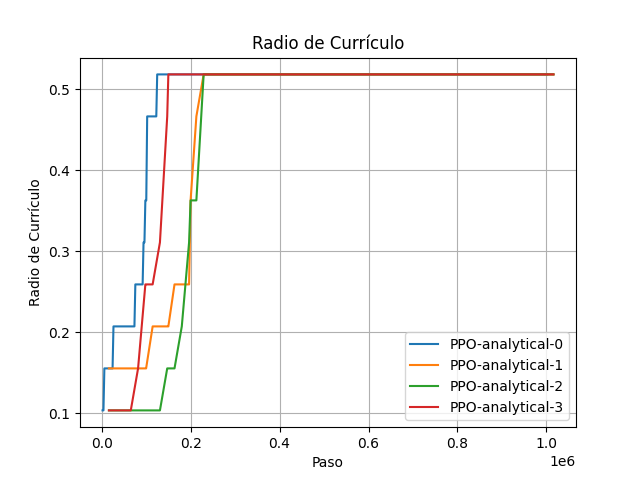
\includegraphics[width=\textwidth]{images/graphs/PPO/Left/curriculum_radius}
		\caption{Entrenamiento con Algoritmo PPO}
		\label{fig:train-ppo-curr-left}
	\end{subfigure}
	\hfill
	\begin{subfigure}[b]{0.48\textwidth}
		\centering
		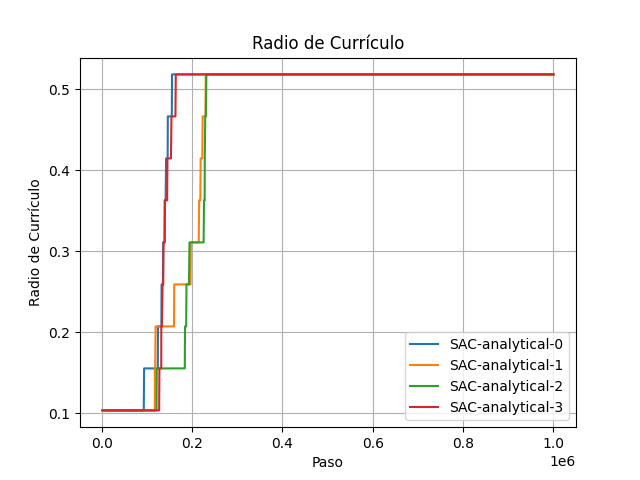
\includegraphics[width=\textwidth]{images/graphs/SAC/Left/curriculum_radius}
		\caption{Entrenamiento con Algoritmo SAC}
		\label{fig:train-sac-curr-left}
	\end{subfigure}
	
	\caption{Evolución del radio de currículo durante el entrenamiento del brazo izquierdo.}
	\label{fig:train-curr-left}
\end{figure}

Con base en las gráficas, es posible apreciar que ambos algoritmos (PPO y SAC) recorrieron la totalidad de las etapas curriculares definidas. De igual manera, un elemento en común entre el comportamiento de ambos algoritmos es que la etapa curricular en la que más tiempo duran es en la última. Esto es esperado en tanto que el radio más amplio es el que genera los casos más difíciles para que la política aprenda. Por eso es, de hecho, un comportamiento deseado pues permanece aprendiendo sobre objetivos difíciles más tiempo.\\

De manera particular, el entrenamiento con PPO muestra un incremento curricular apreciablemente más lento con el estudio de Optuna rotulado \emph{PPO-analytical-2}. También es posible apreciar que el estudio que más rápido logra alcanzar el radio máximo de currículo es \emph{PPO-analytical-0}. En contraste, el entrenamiento con SAC muestra comportamientos similares para parejas de estudios en cuanto a la llegada al radio máximo de currículo, siendo los estudios \emph{SAC-analytical-0} y \emph{SAC-analytical-3} los que lo alcanzan primero.\\

\begin{figure}[h!]
	\centering
	
	\begin{subfigure}[b]{0.48\textwidth}
		\centering
		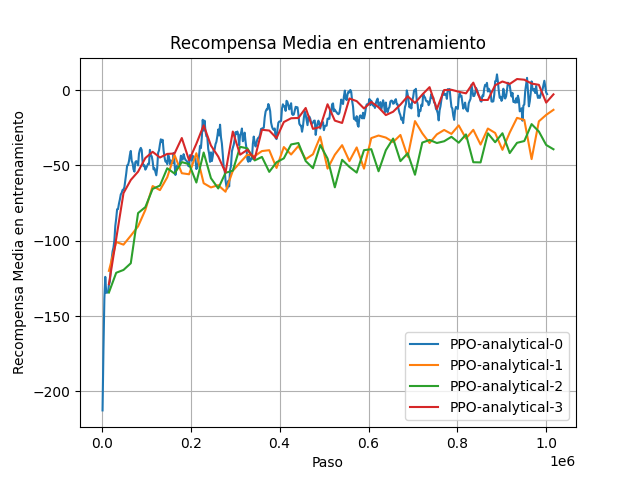
\includegraphics[width=\textwidth]{images/graphs/PPO/Left/ep_rew_mean}
		\caption{Entrenamiento con Algoritmo PPO}
		\label{fig:train-ppo-rew-left}
	\end{subfigure}
	\hfill
	\begin{subfigure}[b]{0.48\textwidth}
		\centering
		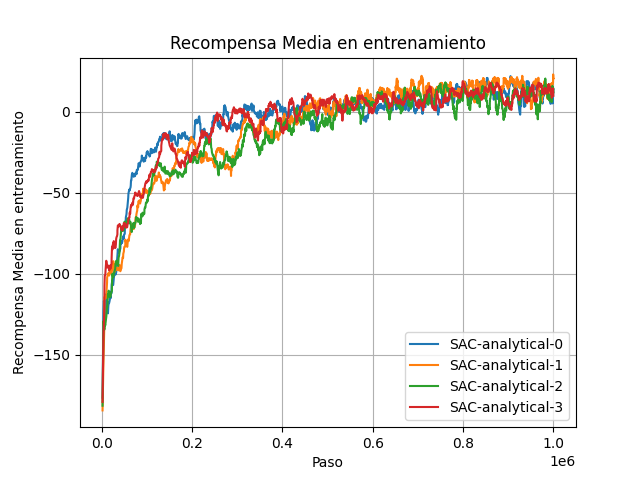
\includegraphics[width=\textwidth]{images/graphs/SAC/Left/ep_rew_mean}
		\caption{Entrenamiento con Algoritmo SAC}
		\label{fig:train-sac-rew-left}
	\end{subfigure}
	
	\caption{Evolución de la media móvil de la recompensa durante el entrenamiento del brazo izquierdo.}
	\label{fig:train-rew-left}
\end{figure}

La evolución de la media móvil de la recompensa permite apreciar que, para el caso de los entrenamientos con PPO, los estudios 0 y 3 presentan una tendencia al incremento del valor de dicho promedio. Si bien estos dos estudios entrenan una política cuya recompensa logra alcanzar el cero y llegar a valores positivos, los otros dos estudios parecen tener una tendencia más plana y estancarse en torno a recompensas cercanas en el intervalo $(-50, 0)$, pero negativas al fin y al cabo.\\

Por su lado, para el entrenamiento con el algoritmo SAC, los cuatro estudios tienen una tendencia y comportamiento similar. Cabe resaltar que tienden a estabilizarse en un valor positivo y que esta llegada sucede en una menor cantidad de timesteps que en el caso de PPO. Para SAC, se supera el cero en torno a los 600.000 timesteps, toda vez que en PPO esto sucede en los dos estudios mencionados apenas hasta los 900.000 timesteps aproximadamente. Esto sugiere que las políticas entrenadas con SAC parecen ser más apropiadas y eficientes para la tarea de aprendizaje propuesta en este proyecto.\\

\begin{figure}[h!]
	\centering
	
	\begin{subfigure}[b]{0.48\textwidth}
		\centering
		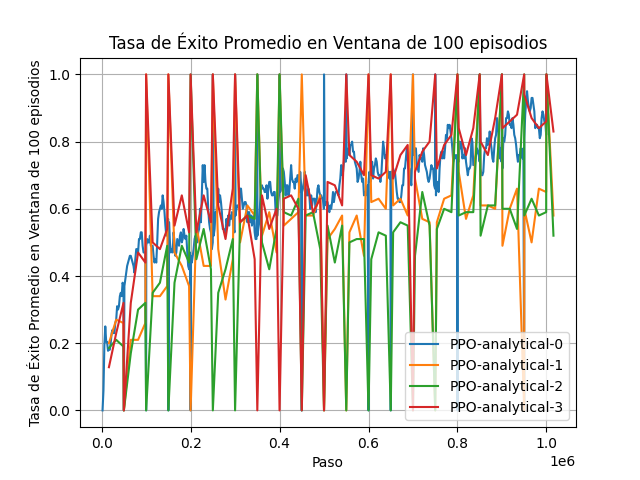
\includegraphics[width=\textwidth]{images/graphs/PPO/Left/success_rate}
		\caption{Entrenamiento con Algoritmo PPO}
		\label{fig:train-ppo-succ-left}
	\end{subfigure}
	\hfill
	\begin{subfigure}[b]{0.48\textwidth}
		\centering
		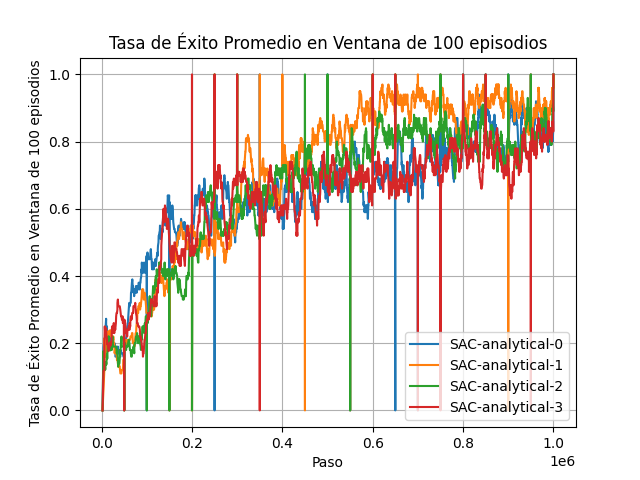
\includegraphics[width=\textwidth]{images/graphs/SAC/Left/success_rate}
		\caption{Entrenamiento con Algoritmo SAC}
		\label{fig:train-sac-succ-left}
	\end{subfigure}
	
	\caption{Evolución de la tasa de éxito durante el entrenamiento del brazo izquierdo.}
	\label{fig:train-succ-left}
\end{figure}

Las gráficas que recopilan la tasa de éxito en episodios de evaluación parcial muestra picos extremos para los dos entrenamientos. Sin embargo, es posible apreciar que la aparición de dichos picos que tienden a irse a 1.0 o a 0.0 son más frecuentes para PPO. Así mismo, los estudios 1 y 2 de PPO nuevamente tienen una tendencia menor al éxito sobre ventanas de 100 episodios consecutivos que los estudios 0 y 3, reiterando nuevamente la hipótesis que los hiperparámetros sintonizados por Optuna para estos últimos estudios les permitieron desempeñarse mejor en el aprendizaje. \\

En el caso del entrenamiento con SAC, si bien la tendencia es similar para los cuatro estudios, se puede apreciar que a medida que incrementa la cantidad de timesteps, los escenarios de evaluación de éxitos consecutivos tienden a ser mayores para el estudio \emph{SAC-analytical-1}. Esto sugiere que dicho estudio es el que tiende a generar mayor cantidad de éxitos y, por ende, correspondería a la mejor política de este algoritmo. \\

La hipótesis resulta ser correcta para el caso del entrenamiento con SAC, pues Optuna arroja que el estudio 1 es el mejor en términos del valor medio de la recompensa. Para el caso de PPO, el mejor estudio es el 3, efectivamente uno de los que logró superar el umbral del cero en el valor de la recompensa media. El valor de la mejor recompensa de cada uno es:

\begin{itemize}
	\item \texttt{PPO-analytical-3}: $-16.07423210144043$
	\item \texttt{SAC-analytical-1}: $10.152339935302734$\\
\end{itemize}

Las siguientes tablas resumen los hiperparámetros sintonizados mediante HPO para cada algoritmo:\\

\begin{table}[h!]
	\centering
	\caption{Hiperparámetros del estudio \texttt{PPO-analytical-3}}
	\begin{tabular}{|l|l|}
		\hline
		\textbf{Hiperparámetro} & \textbf{Valor} \\
		\hline
		Batch size (\texttt{batch\_size})       & 128 \\
		Rango de clip (\texttt{clip\_range})    & 0.2560204063533433 \\
		Coeficiente de entropía (\texttt{ent\_coef}) & 1.5204688692198897e-06 \\
		\(\lambda\) de GAE (\texttt{gae\_lambda})     & 0.9258792340272566 \\
		Factor de descuento (\texttt{gamma})          & 0.9258521201618417 \\
		Tasa de aprendizaje (\texttt{learning\_rate}) & 7.591104805282687e-05 \\
		Pasos por actualización (\texttt{n\_steps})   & 2048 \\
		Coeficiente VF (\texttt{vf\_coef})            & 0.5920392514089517 \\
		\hline
	\end{tabular}
	\label{tab:ppo-analytical-3}
\end{table}

\begin{table}[h!]
	\centering
	\caption{Hiperparámetros del estudio \texttt{SAC-analytical-1}}
	\begin{tabular}{|l|l|}
		\hline
		\textbf{Hiperparámetro} & \textbf{Valor} \\
		\hline
		Batch size (\texttt{batch\_size})       & 512 \\
		Tamaño de buffer (\texttt{buffer\_size}) & 300\,000 \\
		Factor de descuento (\texttt{gamma})    & 0.9199474108376201 \\
		Pasos de gradiente (\texttt{gradient\_steps}) & 8 \\
		Tasa de aprendizaje (\texttt{learning\_rate}) & 7.309539835912905e-05 \\
		Constante de mezcla (\texttt{tau})      & 0.04033291826268561 \\
		Frecuencia de entrenamiento (\texttt{train\_freq}) & 16 \\
		\hline
	\end{tabular}
	\label{tab:sac-analytical-1}
\end{table}

A continuación, se muestra una comparación de las gráficas de métricas correspondientes entre algoritmos diferentes para el agente que modela el brazo derecho.\\

Partiendo por el radio de currículo, el comportamiento en este caso es semejante a lo observado para el brazo izquierdo. Esto sugiere que, si bien pueda haber algunos estudios mejores que otros, al menos en términos del recorrido e incremento curricular, todos se desempeñaron de manera deseable, tanto para el entrenamiento con PPO como con SAC. Esto debido a que todos los estudios alcanzan el radio de currículo máximo y es en este que dura el entrenamiento por la mayor cantidad de tiempo, como se muestra en la Figura \ref{fig:train-curr-right}.\\

\begin{figure}[h!]
	\centering
	
	\begin{subfigure}[b]{0.48\textwidth}
		\centering
		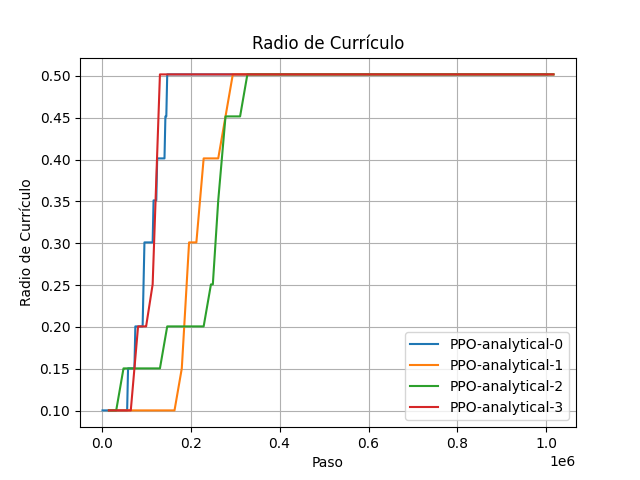
\includegraphics[width=\textwidth]{images/graphs/PPO/Right/curriculum_radius}
		\caption{Entrenamiento con Algoritmo PPO}
		\label{fig:train-ppo-curr-right}
	\end{subfigure}
	\hfill
	\begin{subfigure}[b]{0.48\textwidth}
		\centering
		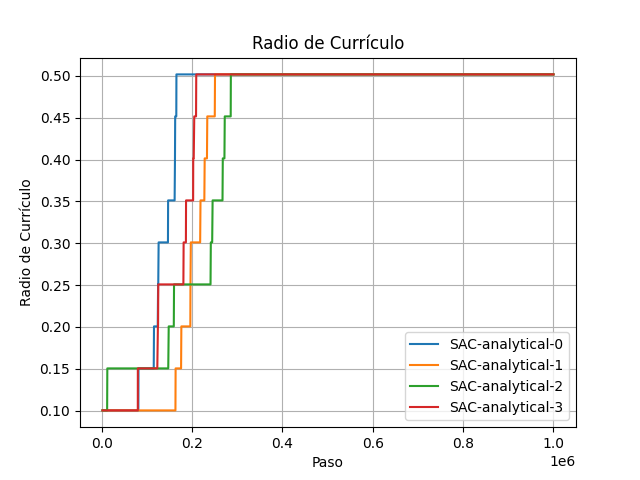
\includegraphics[width=\textwidth]{images/graphs/SAC/Right/curriculum_radius}
		\caption{Entrenamiento con Algoritmo SAC}
		\label{fig:train-sac-curr-right}
	\end{subfigure}
	
	\caption{Evolución del radio de currículo durante el entrenamiento del brazo derecho.}
	\label{fig:train-curr-right}
\end{figure}

Con respecto a la evolución de la media de la recompensa, el entrenamiento se desarrolló de forma análoga al del brazo izquierdo. Sin embargo, vale la pena revisar que el estudio \emph{PPO-analytical-0} parece tener un incremento más pronunciado y que logra acercarse al cero como se aprecia en la Figura \ref{fig:train-ppo-rew-right}, por lo que destaca como un posible candidato a generar la mejor política. Para el entrenamiento con SAC mostrado en la Figura \ref{fig:train-sac-rew-right}, no se puede apreciar de manera clara una política que sea mejor que otra pues todas presentan una tendencia a incrementar la recompensa y estabilizarse en torno a valores positivos.

\begin{figure}[h!]
	\centering
	
	\begin{subfigure}[b]{0.48\textwidth}
		\centering
		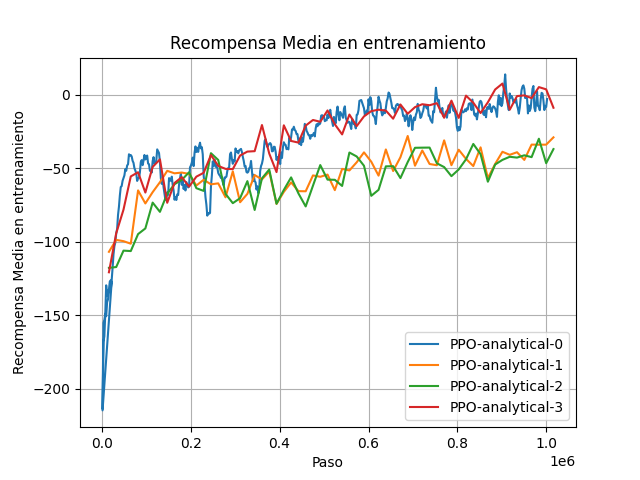
\includegraphics[width=\textwidth]{images/graphs/PPO/Right/ep_rew_mean}
		\caption{Entrenamiento con Algoritmo PPO}
		\label{fig:train-ppo-rew-right}
	\end{subfigure}
	\hfill
	\begin{subfigure}[b]{0.48\textwidth}
		\centering
		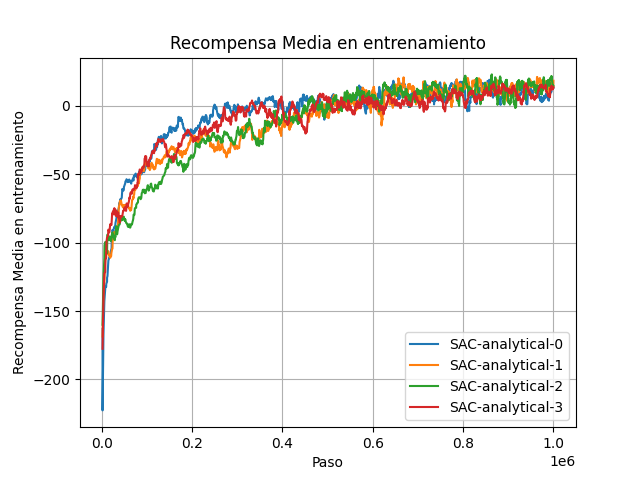
\includegraphics[width=\textwidth]{images/graphs/SAC/Right/ep_rew_mean}
		\caption{Entrenamiento con Algoritmo SAC}
		\label{fig:train-sac-rew-right}
	\end{subfigure}
	
	\caption{Evolución de la media móvil de la recompensa durante el entrenamiento del brazo derecho.}
	\label{fig:train-rew-right}
\end{figure}

Las gráficas que muestran la tasa de éxito con los timesteps son particularmente más caóticas que las generadas para el brazo izquierdo. Específicamente, para PPO (Figura \ref{fig:train-ppo-succ-right}) se generan con mayor frecuencia picos de éxitos consecutivos y de fracasos consecutivos, siendo el estudio 3 el que tiene las disparidades más pronunciadas de todos. De cualquier manera, el mismo patrón ascendente se observa para los estudios 0 y 1. \\

En el caso de SAC mostrado en la Figura \ref{fig:train-sac-succ-right}, resulta destacable que los estudios 0 y 2 tienen picos de éxitos consecutivos relativamente temprano, antes de los 200.000 timesteps. De cualquier manera, el patrón ascendente se observa para los cuatro estudios, siendo los estudios 1 y 2 los que parecen tener la tendencia más cercana a 1.0 al finalizar el periodo de entrenamiento.\\

\begin{figure}[h!]
	\centering
	
	\begin{subfigure}[b]{0.48\textwidth}
		\centering
		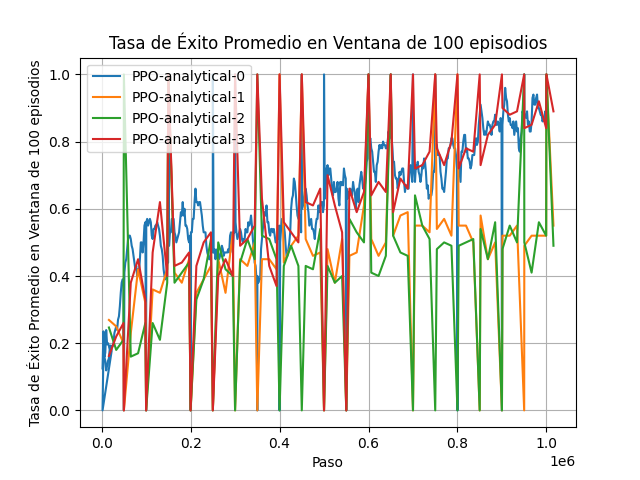
\includegraphics[width=\textwidth]{images/graphs/PPO/Right/success_rate}
		\caption{Entrenamiento con Algoritmo PPO}
		\label{fig:train-ppo-succ-right}
	\end{subfigure}
	\hfill
	\begin{subfigure}[b]{0.48\textwidth}
		\centering
		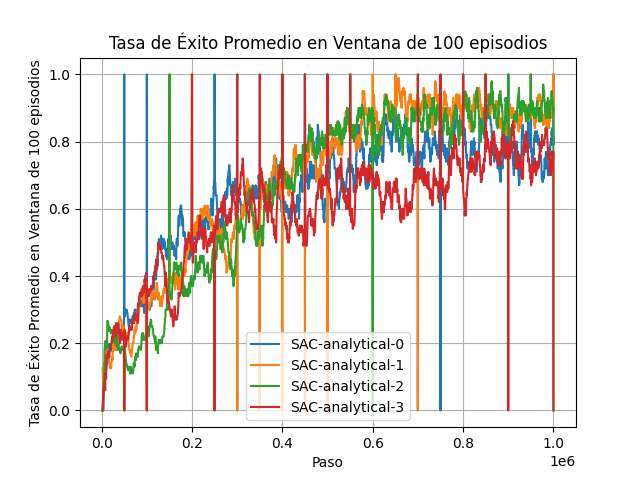
\includegraphics[width=\textwidth]{images/graphs/SAC/Right/success_rate}
		\caption{Entrenamiento con Algoritmo SAC}
		\label{fig:train-sac-succ-right}
	\end{subfigure}
	
	\caption{Evolución de la tasa de éxito durante el entrenamiento del brazo derecho.}
	\label{fig:train-succ-right}
\end{figure}

El proceso de HPO de Optuna arrojó que, para el brazo derecho, los mejores hiperparámetros son los que corresponden a los estudios 3 de PPO y 2 de SAC. El valor de la mejor recompensa de cada uno es:

\begin{itemize}
	\item \texttt{PPO-analytical-3}: $-10.97317123413086$
	\item \texttt{SAC-analytical-2}: $18.295637130737305$\\
\end{itemize}

Puesto que ya se han presentado los hiperparámetros de PPO-3, los de SAC-2 son los siguientes:


\begin{table}[h!]
	\centering
	\caption{Hiperparámetros del estudio \texttt{SAC-analytical-2}}
	\begin{tabular}{|l|l|}
		\hline
		\textbf{Hiperparámetro} & \textbf{Valor} \\
		\hline
		Batch size (\texttt{batch\_size})        & 256 \\
		Tamaño de buffer (\texttt{buffer\_size}) & 300\,000 \\
		Factor de descuento (\texttt{gamma})     & 0.9258521201618417 \\
		Pasos de gradiente (\texttt{gradient\_steps}) & 1 \\
		Tasa de aprendizaje (\texttt{learning\_rate}) & 4.066563313514796e-05 \\
		Constante de mezcla (\texttt{tau})       & 0.045919418093545196 \\
		Frecuencia de entrenamiento (\texttt{train\_freq}) & 1 \\
		\hline
	\end{tabular}
	\label{tab:sac-analytical-2}
\end{table}
